\documentclass[11pt,a4paper]{article}

\usepackage[spanish]{babel}
\usepackage{amsmath,amsfonts, amssymb, amsthm} % Podemos añadir amssymb, amsthm o bm
\usepackage{graphicx, tikz, xparse, array}
\usepackage[top=2cm,bottom=2cm,left=3cm,right=3cm,marginparwidth=1.75cm]{geometry} % Este paquete permite modificar los márgenes del documento
\usepackage[colorlinks=true, allcolors=blue]{hyperref} % Se indica que los hipervínculos van todos en azul
\usepackage{setspace}
\usepackage{caption}
\usepackage{xcolor}
\usepackage{graphicx} % Paquete para incluir imágenes
\usepackage{fancyhdr} % Paquete para cabeceras y pies de página
\usepackage{lipsum}   % Para generar texto de ejemplo
\usepackage[most]{tcolorbox}

\tcbuselibrary{breakable}


%Colores
\definecolor{verdeSuave}{HTML}{6AD58A}
\definecolor{verdeFuerte}{HTML}{206936}
\definecolor{blanco}{HTML}{FFFFFF}
\definecolor{negro}{HTML}{000000}
\definecolor{azulSuave}{HTML}{6ac9d5}
\definecolor{naranjaSuave}{HTML}{d5c06a}
\definecolor{rojoSuave}{HTML}{EF4949}
\definecolor{amarilloSuave}{HTML}{D8E058}


\setstretch{1.2}
\decimalpoint


%\graphicspath{ {images/}}

\title{\textbf{Tema 1: } Teoría de curvas}
\author{Mateo Rama García}


%\date{Fecha}

\begin{document}
  
\begin{titlepage}
  \centering  
  \vspace*{1cm}  % Espacio opcional antes de la imagen
  
\includegraphics[width=0.3\textwidth]{uniovi.jpg} \hspace{2cm}
  
\includegraphics[width=0.3\textwidth]{descarga.jpeg} \\[1cm] 
  \vspace{\fill}% Imagen centrada arriba
  \hrule
  \vspace{0.5cm}
  {\Huge \bfseries Trabajo en grupo\par}
  \vspace{0.5cm}
  {\Large \bfseries Fase II\par}
  \vspace{0.5cm}
  \hrule
  \vspace{1cm}
  {\bfseries PL3-B \\ [3ex]
  Andrés Fernández-Junquera Fernández UO302806\\[3ex]
  Bruno Martín Rivera UO302144\\[3ex]
  Javier Ortín Rodenas UO299855\\[3ex]
  Mateo Rama García UO300710\par} % Nombres centrados
  \vspace{\fill}  % Espacio después de los nombres
  {\Large \textbf{Fundamentos de computadores y redes}\par}
\end{titlepage}



\newpage

\tableofcontents

\newpage


\section{Descifrar entradas válidas}
En esta primera parte, se describirían los pasos que se llevaron a cabo por parte de los intengrantes 
del grupo para descifrar las entradas válidas de cada una de las Stages. 
\vspace{2ex}

Para descifrar cualquiera de las entradas válidas, se utilizó el 
modo depuración que nos ofrece \texttt{Visual Studio 2022}. Para ello, abrimos el 
archivo \texttt{main.exe} y ejecutamos en modo depuración. Haciendo click derecho, 
seleccionamos la opción ir al desensamblado. Una vez allí, avanzamos las diferentes sentencias 
en ensamblador con \texttt{F10} hasta llegar a la sentencia de ensamblador en la que 
se llama a la función \texttt{Stage()} correspondiente, pulsamos \texttt{F11} para acceder 
al código de está función en lenguaje ensamblador.

\subsection{Stage1()}
Una vez hemos pulsado \texttt{F11} en la llamada a la función \texttt{Stage1()}, 
nos encontramos con el siguiente fragmento de código en ensamblador:
\begin{center}
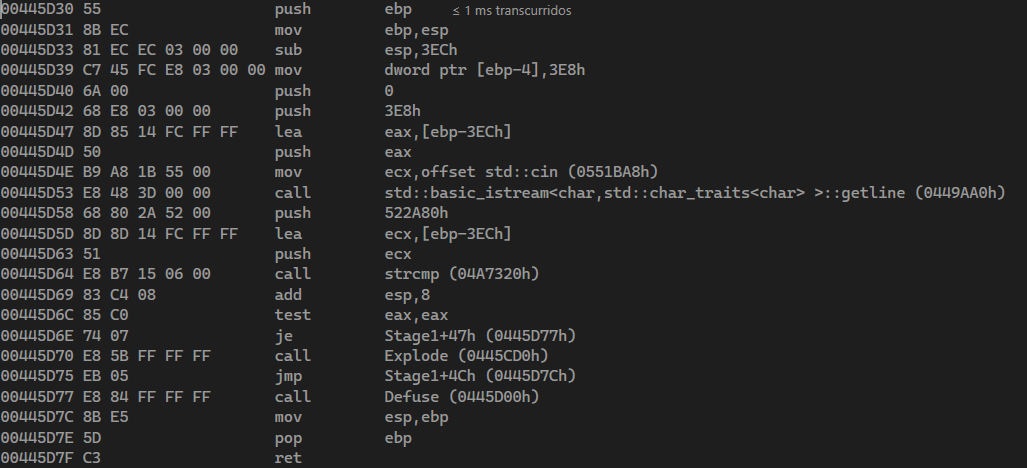
\includegraphics[width=\textwidth]{Stage1/Stage1.png}
\end{center}

Al observar este fragmento de código, podemos observar que la llamada a la función 
\texttt{Explode()} se encuentra en la dirección de memoria \texttt{00445D70h} y la llamada 
a la función \texttt{Defuse()} se encuentra en la dirección \texttt{00445D77h}. 
\vspace{2ex}

En nuestro caso, queremos desactivar la bomba, por tanto solo nos interesa la función 
\texttt{Defuse()}. Para ello buscamos, una instrucción en ensamblador que sea un salto condicional 
a la dirección de memoria de la función \texttt{Defuse()}.


\begin{center}
  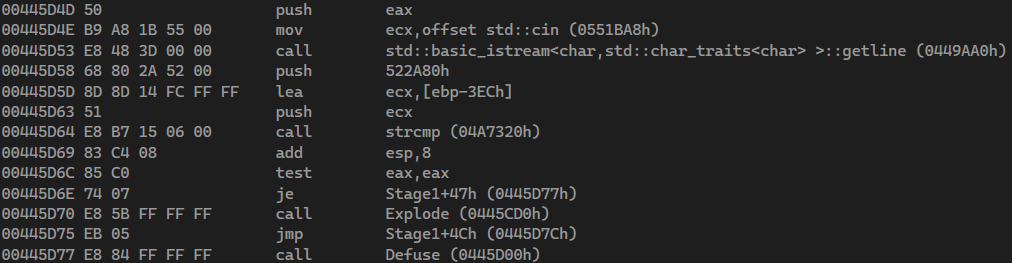
\includegraphics[width=\textwidth]{Stage1/SaltoStage1.png}
\end{center}

Como se muestra en la anterior imagen el salto condicional a la función \texttt{Defuse()} esta almacenado 
en la dirección de memoria \texttt{00445D6Eh}. Este salto es del tipo \texttt{JE} es decir, salta en caso 
de que sean iguales los dos valores que se comparan. Si observamos, las lineas de código anteriores, 
podemos ver que se realizar un \texttt{test eax, eax}, la cual es una instrucción que realiza un AND y 
solo modifica la Zero Flag. Esta instrucción solo activará la Zero Flag si el resultado el registro \texttt{eax} es 0.
\vspace{2ex}

  Sabemos que el registro \texttt{eax} se usa 
normalmente para almacenar el resultado de operaciones aritméticas o llamadas a funciones. En nuestro caso, 
como se puede observar arriba se realiza la llamada a la función \texttt{strcmp()}. Por tanto,  
\texttt{eax} almacenará el valor que retorne está función, la cuál devuelve 0 si son iguales las dos cadenas comparadas y un valor distinto en caso contrario. 
\vspace{2ex}

Para llamar a la función \texttt{strcmp()} se necesitan pasar dos cadenas en forma de parámetro a través de la pila, 
por tanto debemos observar las instrucciones superiores con el objetivo de observar los distintos \texttt{push} que se realizan. 
\vspace{2ex}

Podemos observar, que se llama a la función \texttt{cin.getLine()} para almacenar la cadena 
que el usuario introduce por teclado. Esta función almacena la cadena a partir de la dirección de memoria 
que se encuentra almacenada en el registro \texttt{eax}, ya que anteriormente se realiza la instrucción \texttt{push eax}.
\vspace{2ex}

A continuación, se mueve la dirección de memoria en la que se encuentra almacenada la cadena introducida por el usuario 
al registro \texttt{ecx} y se realiza un \texttt{push ecx} para pasarla como parámetro a la función \texttt{strcmp()}. 
\vspace{2ex}

En las líneas de código superiores, también se puede observar que 
se realiza un \texttt{push 522A80h}, la cual es el otro parámetro que se le pasa a \texttt{strcmp()}. Por tanto, podemos deducir 
que se trata de la dirección de memoria que contiene el primer carácter la cadena con la que se va a realizar 
la comparación y la cuál es la que tenemos que averiguar, para desactivar la bomba. Ayudándonos de Visual Studio 2022, 
buscamos la dirección de memoria \texttt{522A80h} y nos encontramos con los carácteres codificados en código ASCII, como se muestra en la imagen.

\begin{center}
  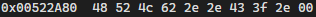
\includegraphics[width=\textwidth]{Stage1/cadenaStage1.png}
\end{center}

En esta dirección de memoria, seleccionamos los bytes hasta el terminador de la cadena, la cual 
es un \textbackslash{}\(0\) y lo traducimos de ASCII a lenguaje natural, 
obteniendo la siguiente cadena:
\begin{center}
\texttt{HRLb..C?.}
\end{center}

Por último, comprobamos que la cadena obtenida es correcta, como se muestra en la siguiente imagen.
\begin{center}
  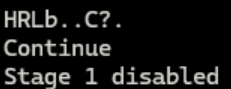
\includegraphics[width=0.3\textwidth]{Stage1/Stage1Correcto.png}
\end{center}

\newpage

\subsection{Stage2()}
Una vez hemos pulsado \texttt{F11} en la llamada a la función \texttt{Stage2()}, nos encontramos con el siguiente fragmento de código 
en ensamblador:
\begin{center}
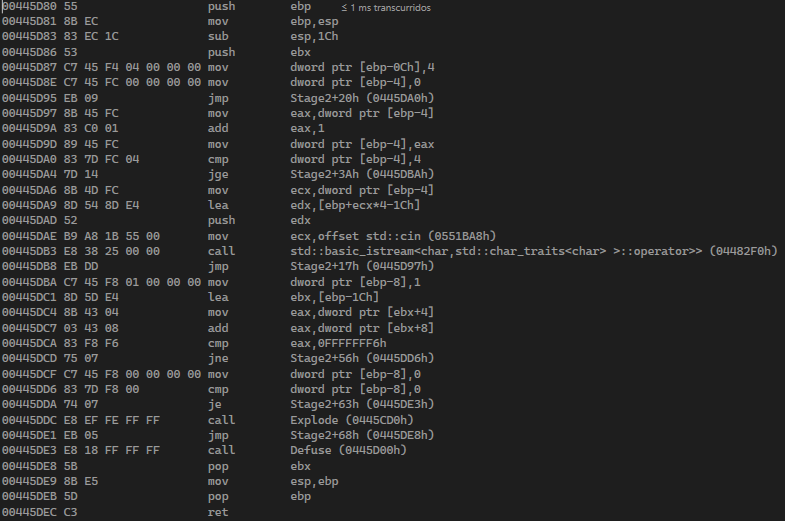
\includegraphics[width=\textwidth]{Stage 2/codigoStage2.png}
\end{center}

Al igual que para el \texttt{Stage1()}, podemos observar que en la dirección de memoria 
\texttt{00445DE3h} se encuentra la llamada a la función \texttt{Defuse()}, la cuál es 
la que nos interesa. En este caso, la estrategia será diferente, no empezaremos de atrás hacia delante, sino 
que primero leeremos el código ensamblador para poder entenderlo y así poder descifrar 
las entradas válidas. 
\vspace{2ex}

Observando el código, podemos ver que se realiza un bucle en el que en cada iteración el
usuario debe introducir un número, los cuáles se almacenan en las direcciones de memoria 
\texttt{ebp+ecx*4-1Ch}, donde el registro \texttt{ecx} en esta instrucción se encarga de almacenar 
el número de iteración en la que se encuentra el bucle. 
\vspace{2ex}

Una vez el bucle ha finalizado y el usuario ha introducido los 4 números, se mueve a la dirección de memoria 
\texttt{ebp-8} el valor 1. En la siguiente instrucción, se realiza un \texttt{lea ebx,[ebp - 1Ch]}. Así, el 
registro \texttt{ebx} almacenará la dirección de memoria correspondiente a la dirección de memoria donde 
se encuentra almacenado el primer número introudicdo por el usuario. En las dos siguientes instrucciones se 
mueve al registro \texttt{eax} el segundo valor introducido por el usuario y se suma en este mismo registro 
el tercer número introducido por el usuario, como se muestra en la siguiente imagen.

\begin{center}
  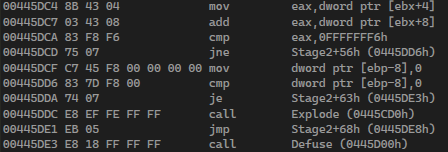
\includegraphics[width=\textwidth]{Stage 2/ultimoStage2.png}
\end{center}

Tras realizar la suma, compara el valor de la suma con el valor \texttt{0FFFFFFF6h} el cual 
es \texttt{-10} en decimal. En caso de que sean iguales, el salto condicional que se encuentra 
en la siguiente linea (\texttt{jne Stage2+56h (0445DD6h)}) no se verifica y por tanto las dos siguientes instrucciones se ejecutan. 
Estas, simplemente mueven el valor 0 a la dirección de memoria \texttt{ebp-8} y compara el valor 
de esta dirección de memoria con el valor \texttt{0}. Lo cual es verdad siempre, así finalmente se cumple la siguiente 
sentencia \texttt{jmp Stage2+63h (00445DE3h)} que es la que llama a la función \texttt{Defuse()}. 
\vspace{2ex}

De esto, concluimos que para desactivar la bomba, el usuario debe introducir 4 números
de forma que la suma del segundo y tercer número sea igual a \texttt{-10}. Procedemos a comprobar 
que esto es así:
\begin{center}
  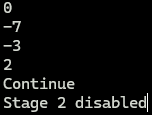
\includegraphics[width=0.3\textwidth]{Stage 2/Stage2Correcto.png}
\end{center}

Notar que en caso de que no sumasen \texttt{-10}, el valor de la dirección de memoria \texttt{ebp-8} no se cambiaría 
y por tanto almacenaría el valor 1. En ese caso, al realizar la comparación con el valor 0 no serían iguales y por 
tanto, se llamaría a la función \texttt{Explode()} y la bomba estallaría.

\vspace{2mm}
\begin{center}
  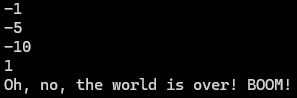
\includegraphics[width=0.4\textwidth]{Stage 2/explode.png}
\end{center}

\newpage
\subsection{Stage3()}
Esta función \texttt{Stage3} nos pide introducir por teclado dos números, así que estudiaremos las características
necesarias de nuestros parámetros para desactivar esta tercera etapa. Al pulsar \texttt{F11} en la función
\texttt{Stage3()} podemos observar la primera parte del código:
\begin{center}
  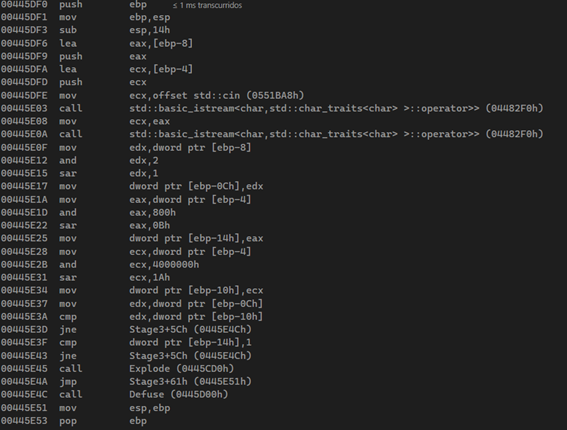
\includegraphics[width=\textwidth]{Stage3/img1.png}
\end{center}

Notamos que la llamada a la función \texttt{Defuse()} se encuentra en la dirección de memoria
\texttt{00445E4Ch}, por lo que veremos cómo llegar a ella paso por paso.

Después de la preparación de la pila (las tres primeras líneas), se leen las 2 entradas por
teclado del usuario. Obsérvese las instrucciones guardadas en las direcciones
\texttt{00445E03h} y \texttt{00445E0Ah}: están ambas leyendo por teclado y se han guardado
los valores de esas entradas en \texttt{[ebp-8]} y \texttt{[ebp-4]}.
\begin{center}
  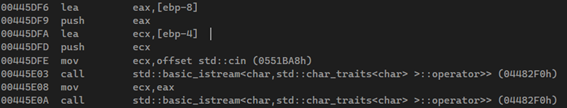
\includegraphics[width=\textwidth]{Stage3/img2.png}
\end{center}
\noindent Con el fin de simplificar la explicación, llamaremos variable 1, 2 y 3 a los
valores que hemos obtenido a partir de los parámetros introducidos por el usuario.

\vspace{2mm}
\textbf{Variable 1:} Se guarda el primer valor introducido en \texttt{edx} y le aplica una
operación \texttt{and} con el valor 2. De este modo, el resultado guardará solo el bit 1
(segundo por la derecha), que tomará el valor 1 si el de la variable era 1 y valdrá 0 si el
de la variable era 0 (el resto de bits valdrán 0 como resultado del \texttt{and}).

Justo después, desplaza esta variable un bit a la derecha (\texttt{sar edx,1}), por lo que la variable
valdrá exactamente 1 o 0, según el valor del bit que originalmente era el número 1.
Guarda este resultado en la dirección de memoria \texttt{ebp-0Ch}.

\vspace{4mm}
\textbf{Variable2:} Ahora, en las instrucciones guardas a partir de la dirección de memoria
\texttt{00445E1Ah}, se trabaja con el segunda número introducida. Se toma su valor y con otra máscara
\texttt{and} y el valor \texttt{800h} (=1000…00b) se comprueba el valor del bit número 11, y se desplaza
hasta el bit número 0.  Se guarda este valor en la dirección de memoria \texttt{ebp-14h}. 
\begin{center}
  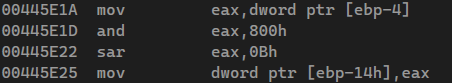
\includegraphics[width=\textwidth]{Stage3/img4.png}
\end{center}

\vspace{4mm}
\textbf{Variable3:} Ahora se vuelve a tomar el segundo parámetro originalmente introducido y se
introduce a la variable \texttt{ecx}. Con la máscara \texttt{and ecx,4000000h} se mira si el bit 26 del primer
número es 1 y se vuelve a mover 26 bits a la derecha con la instrucción \texttt{sar}. Se guarda este valor
en la dirección de memoria \texttt{ebp-10h}.
\begin{center}
  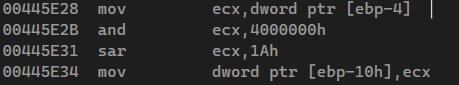
\includegraphics[width=\textwidth]{Stage3/img5.png}
\end{center}

Finalmente, recogemos las variables 1 y 3. La instrucción \texttt{jne} (jump if not equal) hace que la bomba se desactive
(llevando el puntero de dirección a la instrucción que llama a \texttt{Defuse()}) si los dos valores son distintos.
En otro caso, si la variable 2 es distinta a 1 (el bit 11 del segundo parámetro igual a 0) se desactiva también la bomba.
Si no se cumple nada de esto, la bomba explota.

\begin{center}
  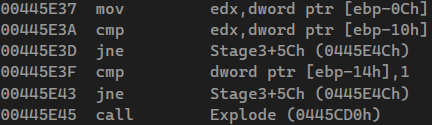
\includegraphics[width=\textwidth]{Stage3/img6.png}
\end{center}

En resumen, para poder desactivar la bomba nos piden que el bit 1 del primer numero y el bit 26 de la segunda sean distintos.
O en su defecto, que el bit 11 de la segunda sea 0.

Notamos que los parámetros deben ser números siempre, de ser caracteres explotará la bomba.

\newpage
\subsection{Stage4()}
Siguiendo el mismo procedimiento que en los casos anteriores, al pulsar \texttt{F11} en la
llamada a \texttt{Stage4()} obtenemos el siguiente código:

\begin{center}
  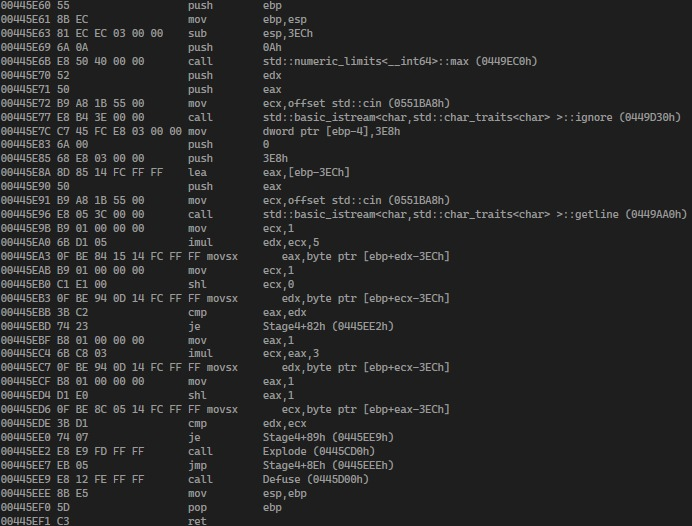
\includegraphics[width=\textwidth]{Stage4/img1.png}
\end{center}

Notamos que las llamadas a \texttt{Defuse()} y \texttt{Explode()} se encuentran en las
direcciones \texttt{445EE9h} y \texttt{445EE2h}, respectivamente. Además, se corresponden
con un salto relativo de \texttt{89h} y \texttt{82h} (respectivamente) desde la etiqueta
\texttt{Stage4}. Conocer el valor de estos saltos relativos nos sirve de ayuda para comprender
cómo funciona el código. En este caso, explicaremos qué hace el código secuencialmente.

\begin{center}
  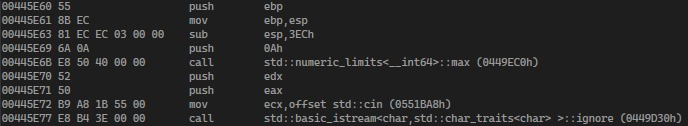
\includegraphics[width=\textwidth]{Stage4/img2.png}
\end{center}

Las tres primeras líneas componen el prólogo del procedimiento, reservando 1004 (\texttt{3ECh}) espacios de pila. A continuación, se llama a \texttt{numeric\_limits::max} para
un entero de 64 bits y obtener así el mayor valor que puede almacenar una variable de este tipo. Sabemos que el registro \texttt{eax} es
comunmente utilizado para dejar los valores de retorno. No obstante, como almacena 32 bits y el valor esperado es de 64, es necesario
utilizar más  espacio para guardar tal valor. Es por ello que también se hace un push de \texttt{edx}, pues estos dos registros contienen en
conjunto el entero de 64 bits correspondiente al máximo posible en un tipo \texttt{\_\_int64}.
\\

A continuación, se apila el valor de este número para que lo utilice. La cuarta línea no apila un parámetro para \texttt{numeric\_limits},
pues esta función no toma parámetros. Se apila \texttt{0Ah} para ser utilizada por \texttt{ignore}, ya que es la codificación del salto de
línea an ASCII. De este modo, se mueve a \texttt{ecx} la dirección de \texttt{cin} y se llama a \texttt{ignore} para que este flujo ignore
las entradas previas hasta encontrar el caracter \texttt{'\textbackslash n'} o llegar al máximo establecido.

\begin{center}
  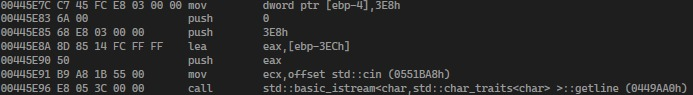
\includegraphics[width=\textwidth]{Stage4/img3.png}
\end{center}

En esta parte se reserva espacio para guardar una cadena de 1000 (\texttt{3E8h}) caracteres como máximo
que será leída por \texttt{getline}. Es por ello que se apila este valor como parámetro (longitud máxima)
junto con la dirección de inicio la cadena (se deja la dirección en \texttt{eax} con \texttt{lea} y se apila
\texttt{eax}). La función \texttt{getline} modificará las direcciones de memoria pertinentes para guardar la
entrada del usuario. Puesto que 0 se corresponde con el código del terminador \texttt{'\textbackslash 0'},
apilar este valor podría servir como delimitador para \texttt{getline}.
\\
\begin{center}
  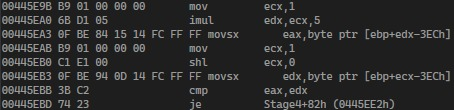
\includegraphics[width=\textwidth]{Stage4/img4.png}
\end{center}

\vspace{2mm}
Una vez leída la cadena, se deja el valor 1 en \texttt{ecx}. Se multiplica
ahora tal valor por 5, dejando el resultado en \texttt{edx}. A continuación,
se accede al índice 5 de la cadena (sexto caracter) y se almacena en \texttt{eax}.
Se realiza un procedimiento análogo al dejar el caracter de índice 1 de la cadena
en \texttt{edx}, pues se desplaza 1 en 0 bits a la izquiera (el resultado es 1).
Finalmente, se compara el contenido de \texttt{eax} con el de \texttt{edx}, saltando
a la llamada a \texttt{Explode} en caso de ser iguales.
\\

\begin{center}
  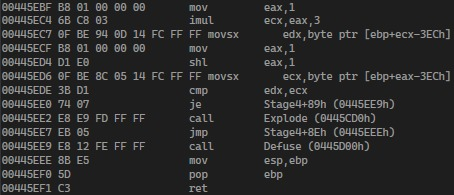
\includegraphics[width=\textwidth]{Stage4/img5.png}
\end{center}

Análogamente, se comparan otros dos caracteres de la clave
introducida por el usuario. El primero es el situado en el índice 3 (resultado
de multiplicar 3 por 1), mientras que el segundo es el de índice 2 (se desplaza
un bit a la izquierda el valor 1, lo que equivale a multiplicarlo por 2). A diferencia
del caso anterior, buscamos que sí coincidan ahora, pues de lo contrario explotaría la bomba.

\vspace{2mm}
Por todo lo anterior, podemos deducir las condiciones que debe cumplir la clave
introducida por el usuario para que la bomba no explote en esta fase. En primer lugar,
cabe recordar que los índices de las cadenas comienzan en 0. Por tanto, para que no explote,
la cadena ha de tener su sexto caracter distinto de su segundo. Además, el cuarto caracter
y el tercero sean iguales. Ambas condiciones han de verificarse simultáneamente, o de lo contrario
la bomba explotará.

\vspace{2mm}
\begin{center}
  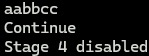
\includegraphics[]{Stage4/img6.png} \\
  \noindent Ejemplo de entrada válida
\end{center}

\vspace{2mm}
\begin{center}
  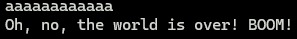
\includegraphics[]{Stage4/img7.png} \\
  \noindent Ejemplo de entrada no válida
\end{center}
\newpage

\section{Modificación del fichero ejecutable}
Para modificar el código de la bomba para que indique que está desactivada sin necesidad de
introducir ninguna entrada, vamos a proceder sustitullendo las instrucciones call de cada Stage
por la instrucción NOP. Vamos a mostrar este procedimiento para Stage1, siendo análogo para las
otras tres fases.

\vspace{2mm}
Primero, abrimos en Visual Studio el archivo main.exe, pulsamos F10 para empezar a depurar y mostramos el desensamblado incluyendo los bytes de código.
\begin{center}
  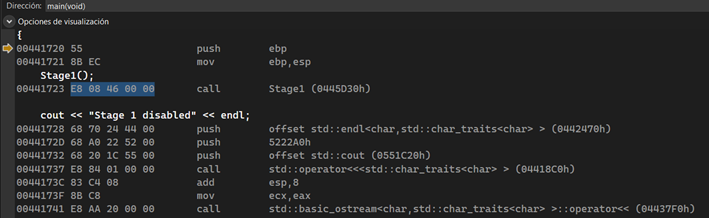
\includegraphics[width=\textwidth]{Modificacion/img1.png}
\end{center}
\noindent Así, podemos ver que la instrucción \texttt{call Stage1} se 
codifica como \texttt{E8 08 46 00 00}.

\vspace{3mm}
Utilizando ahora el programa HxD, abrimos una copia de \texttt{main.exe}.
Para encontrar la llamada a \texttt{Stage1}, pulsamos \texttt{Ctrl+F},
seleccionamos "Valores hexadecimales", y buscamos el valor
\texttt{E8 08 46 00 00}.
\begin{center}
  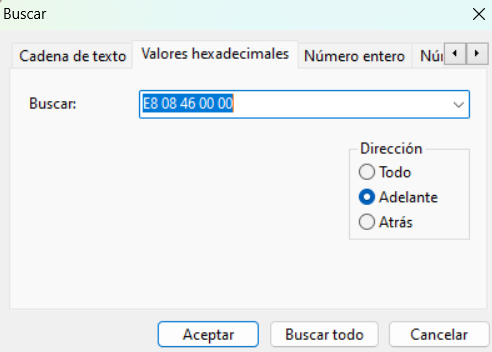
\includegraphics[width=\textwidth]{Modificacion/img2.png}
\end{center}

Tras esto, veremos algo similar a la siguiente pantalla, donde se muestra
esta llamada a \texttt{Stage1} entre el resto de instrucciones de \texttt{main}
codificadas en código máquina y expresadas en hexadecimal.
\begin{center}
  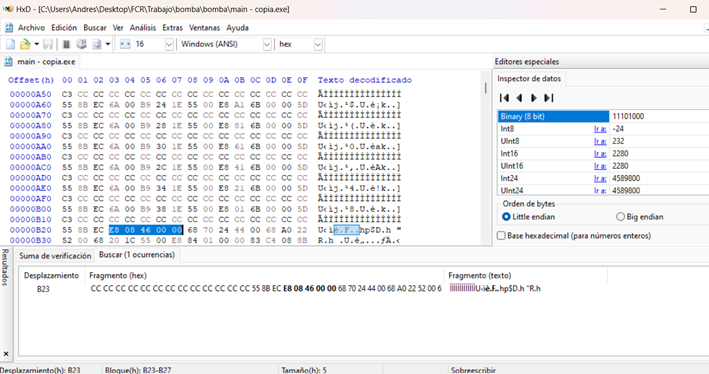
\includegraphics[width=\textwidth]{Modificacion/img3.png}
\end{center}

\noindent Por último, sustituimos estos 5 bytes por la instrucción \texttt{NOP}
en 5 bytes, codificada por la secuencia \texttt{0F 1F 44 00 00}.
\begin{center}
  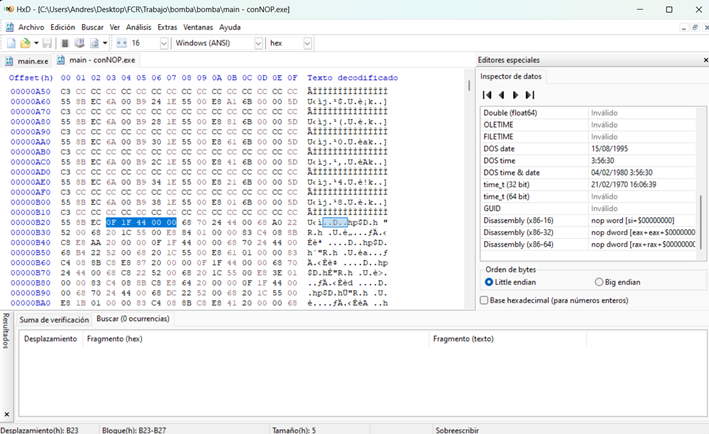
\includegraphics[width=\textwidth]{Modificacion/img4.png}
\end{center}

Repitiendo este procedimiento con \texttt{Stage2}, \texttt{Stage3} y \texttt{Stage4},
conseguiremos que, al ejecutar la función \texttt{main}, se indique que la bomba está
desactivada sin necesidad de introducir ninguna entrada.
\begin{center}
  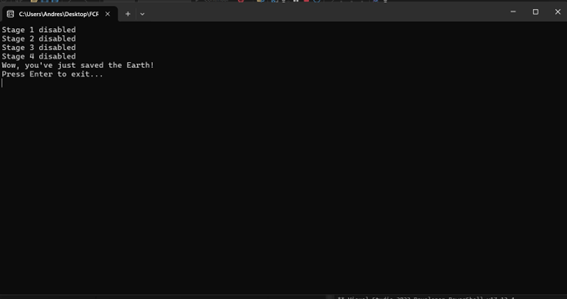
\includegraphics[width=\textwidth]{Modificacion/img5.png}
\end{center}
\newpage

\section{División del trabajo}
\end{document}
